\subsection{放出検知スイッチ・フライトピン}
図\ref{fig3_1_inhibit_d}中のSW1, SW2, SW3は放出検知スイッチであり,放出検知ピンにより開放・短絡が制御される(図\ref{fig3-1pin}).

\begin{figure}[htbp]
	\begin{minipage}{0.32\hsize}
		\centering
		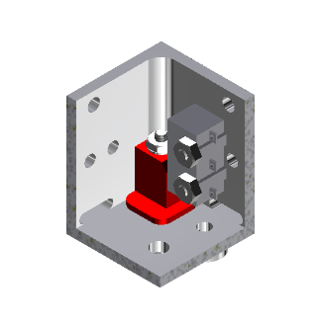
\includegraphics[height=0.7\linewidth]{./03/fig/pin_a.png}
		\subcaption{Oblique View}
	\end{minipage}
	\begin{minipage}{0.32\hsize}
		\centering
		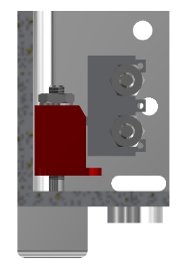
\includegraphics[height=0.7\linewidth]{./03/fig/pin_b.png}
		\subcaption{Pushed State}
	\end{minipage}
	\begin{minipage}{0.32\hsize}
		\centering
		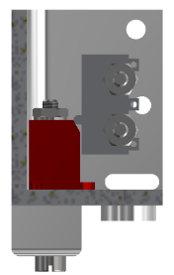
\includegraphics[height=0.7\linewidth]{./03/fig/pin_c.png}
		\subcaption{Released State}
	\end{minipage}
	\caption{Release Detection Pin}
	\label{fig3-1pin}
\end{figure}


放出ポッド搭載までの意図せぬ電源投入を防ぐためにフライトピンを設けた.本衛星には放出検知ピンを機械的にロックするフライトピン(1a,1b,図\ref{fig3-1fpin})と電気的にEPS以降の起動を阻止するフライトピン2がある.

\begin{figure}[htbp]
	\begin{minipage}{\hsize}
		\centering
		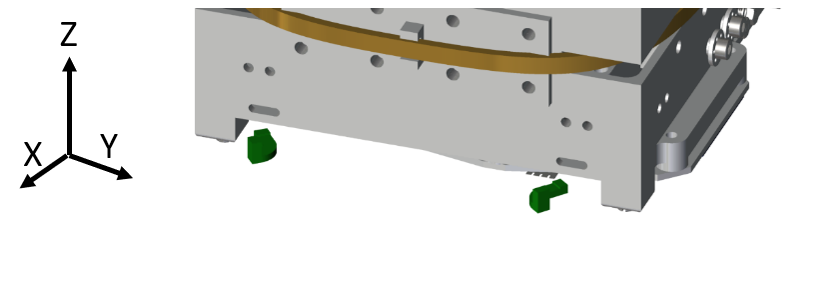
\includegraphics[width=0.5\linewidth]{./03/fig/fpin_a.png}
		\subcaption{Oblique View}
	\end{minipage}\\
	\begin{minipage}{0.5\hsize}
		\centering
		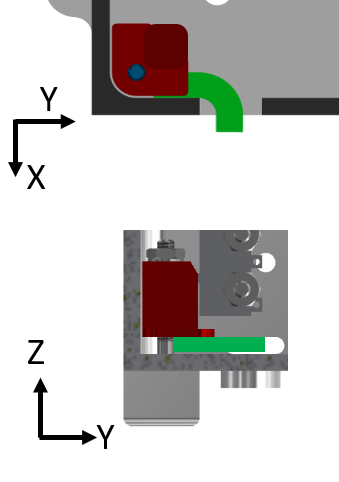
\includegraphics[height=0.7\linewidth]{./03/fig/fpin_b.png}
		\subcaption{Locked State}
	\end{minipage}
	\begin{minipage}{0.5\hsize}
		\centering
		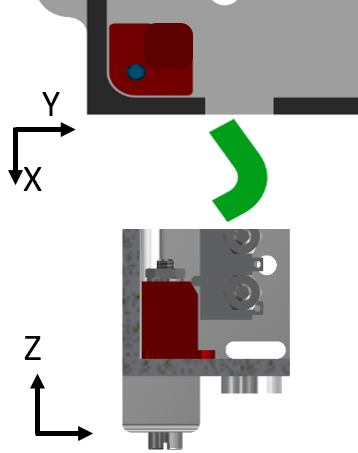
\includegraphics[height=0.7\linewidth]{./03/fig/fpin_c.png}
		\subcaption{Released State}
	\end{minipage}
	\caption{Flight Pin 1}
	\label{fig3-1fpin}
\end{figure}

フライトピン2はEPSの組み込み機能であるSeparation Switch端子とRBF(Remove Before Flight) Switch端子をGNDに導通させることでEPSの起動を防ぐ.

